\documentclass[tikz]{standalone}

\begin{document}
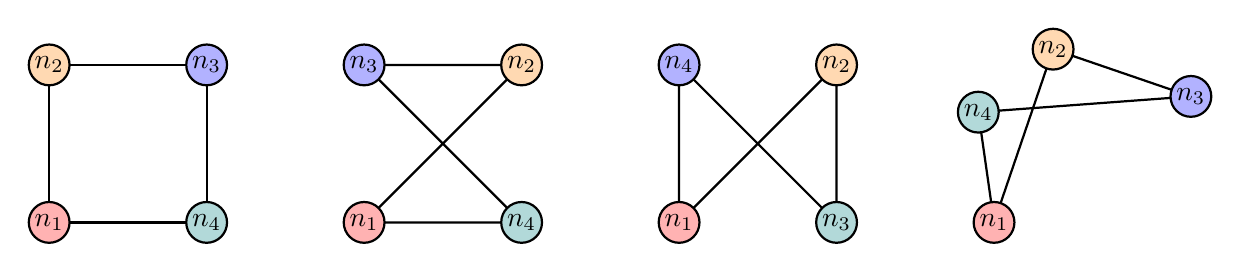
\begin{tikzpicture}[
  vertex/.style = {circle, draw, inner sep=1pt, fill=white},
  vertex1/.style = {vertex, fill=red!30!white},
  vertex2/.style = {vertex, fill=orange!30!white},
  vertex3/.style = {vertex, fill=blue!30!white},
  vertex4/.style = {vertex, fill=teal!30!white},
]

\draw[thick]
  (0,0) node[vertex1] (n1^1) {$n_1$}
  -- (0,2) node[vertex2] (n2^1) {$n_2$}
  -- (2,2) node[vertex3] (n3^1) {$n_3$}
  -- (2,0) node[vertex4] (n4^1) {$n_4$} -- cycle;

\begin{scope}[xshift=4cm]
  \draw[thick]
    (0,0) node[vertex1] (n1^2) {$n_1$}
    -- (2,2) node[vertex2] (n2^2) {$n_2$}
    -- (0,2) node[vertex3] (n3^2) {$n_3$}
    -- (2,0) node[vertex4] (n4^2) {$n_4$} -- cycle;
\end{scope}

\begin{scope}[xshift=8cm]
  \draw[thick]
    (0,0) node[vertex1] (n1^3) {$n_1$}
    -- (2,2) node[vertex2] (n2^3) {$n_2$}
    -- (2,0) node[vertex4] (n3^3) {$n_3$}
    -- (0,2) node[vertex3] (n4^3) {$n_4$} -- cycle;
\end{scope}

\begin{scope}[xshift=12.5cm]
  \draw[thick]
    (-0.5,0) node[vertex1] (n1^4) {$n_1$}
    -- (0.25,2.2) node[vertex2] (n2^4) {$n_2$}
    -- (2,1.6) node[vertex3] (n3^4) {$n_3$}
    -- (-0.7,1.4) node[vertex4] (n4^4) {$n_4$} -- cycle;
\end{scope}
\end{tikzpicture}
\end{document}
